\begin{frame}
\frametitle{Electronic Flight Bags}
\begin{center}
Aeronautical Data and Information
\end{center}
\end{frame}

\begin{frame}
\frametitle{Aeronautical Data and Information}
\begin{block}{Aviation, Navigation and Geodesy}
\begin{itemize}
\item<1-> This part is not technical.
\item<2-> There is no code here.
\item<3-> Only whinging.
\end{itemize}
\end{block}
\end{frame}

\begin{frame}
\frametitle{CASR 175}
\begin{block}{What is CASR 175 about?}
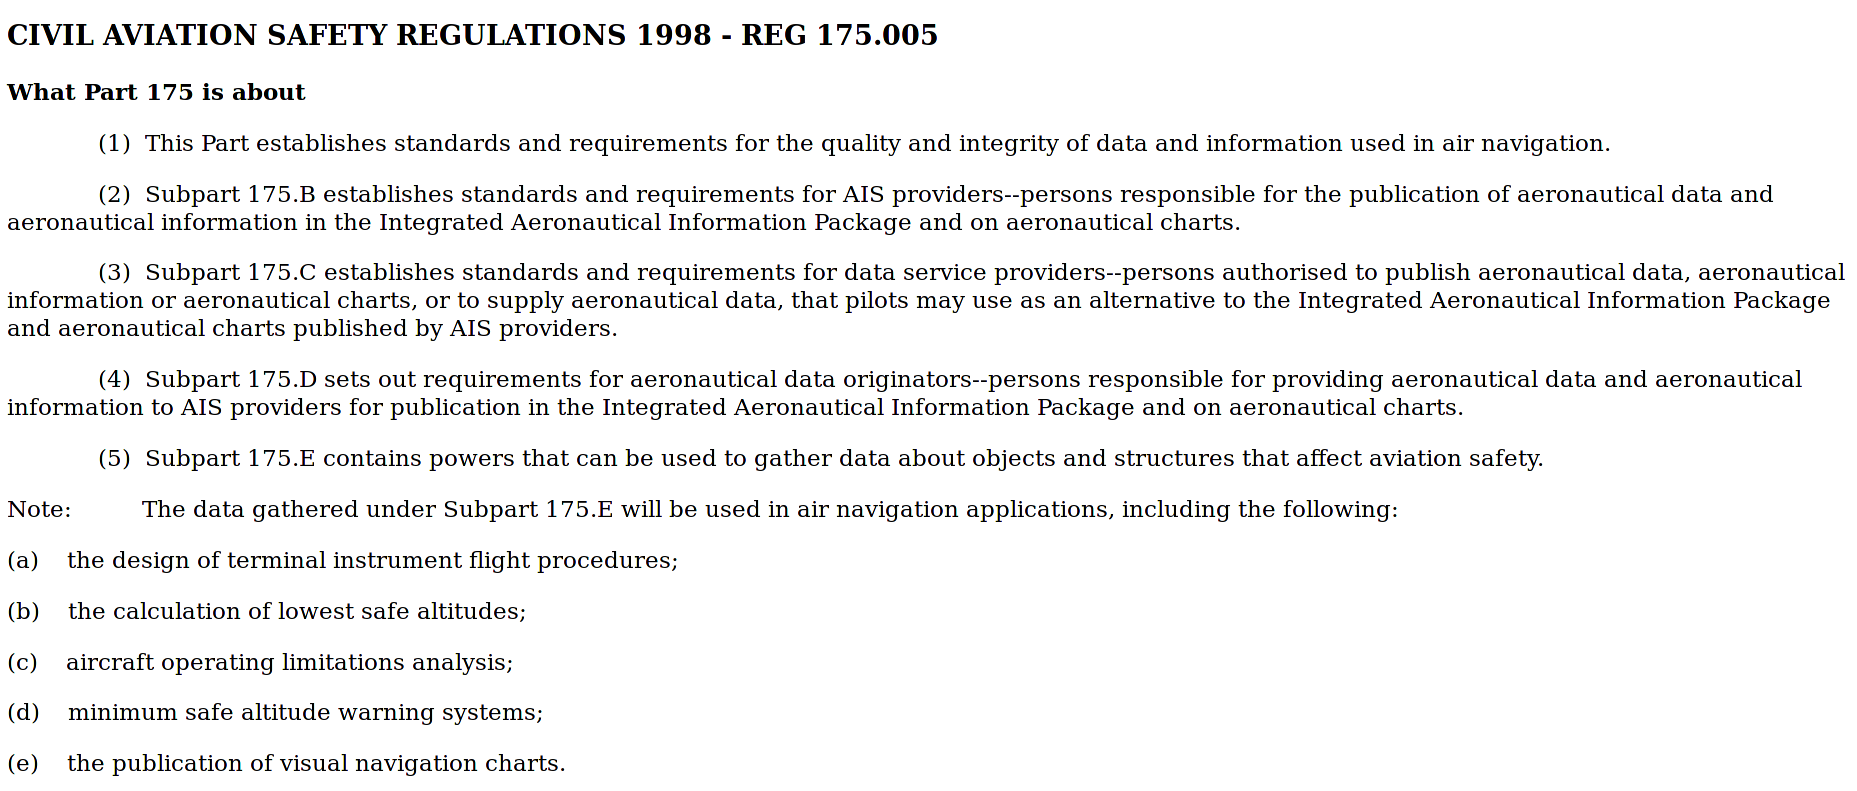
\includegraphics[height=0.5\textheight]{image/casr175_005.png}
\end{block}
\par
``(e) the publication of visual navigation charts.''
\end{frame}

\begin{frame}
\frametitle{CAR 233 (1)(h) \emph{moved to CASR 175}}
\scriptsize
\begin{block}{CAR 233 (1)(h)}
The pilot in command of an aircraft must not commence a flight if he or she has not received evidence, and taken such action as is necessary to ensure, that:
\par
\ldots
\par
(h)  the aeronautical data and aeronautical information mentioned in subregulation (1A) is carried in the aircraft and is readily accessible to the flight crew.
\end{block}
\par
\end{frame}

\begin{frame}
\frametitle{VTC/VNC}
\begin{block}{This is a Visual Terminal Chart}
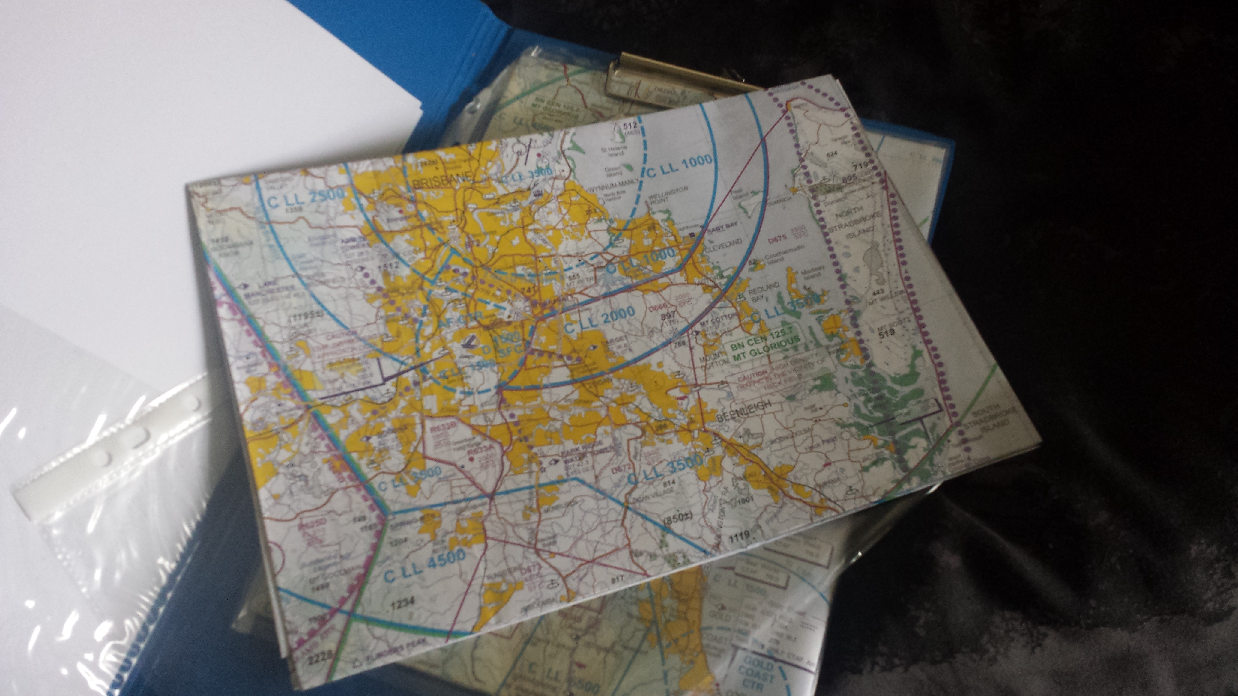
\includegraphics[height=0.3\textheight]{image/vtc.png}
\begin{itemize}
\item<1-> It unfolds out to 500mm x 1000mm.
\item<2-> Updated every 3 months.
\item<3-> Similar to another required chart; VNC.
\end{itemize}
\end{block}
\end{frame}

\begin{frame}
\frametitle{VTC/VNC}
\begin{block}{Surely these exist in electronic format?}
Why yes, they do.
\end{block}
\end{frame}

\begin{frame}
\frametitle{VTC/VNC}
\large
\begin{center}
but
\end{center}
\end{frame}

\begin{frame}
\frametitle{CASR 175.145(1)}
\begin{block}{AIS providers--publication of aeronautical charts relating to areas etc. outside authority}
(1) This regulation applies if an AIS provider publishes an aeronautical chart that includes aeronautical data or aeronautical information that relates to an area, aerodrome, airspace or ATS route not covered by the provider's certificate.
\end{block}
\end{frame}

\begin{frame}
\frametitle{CASR 175.145(1)}
\large
\begin{center}
No problem.
\par
I will use approved electronic AIS aeronautical charts.
\end{center}
\end{frame}

\begin{frame}
\frametitle{CASR 175.145(1)}
\large
\begin{center}
but
\end{center}
\end{frame}

\begin{frame}
\frametitle{CASR 175.145(1)}
\begin{center}
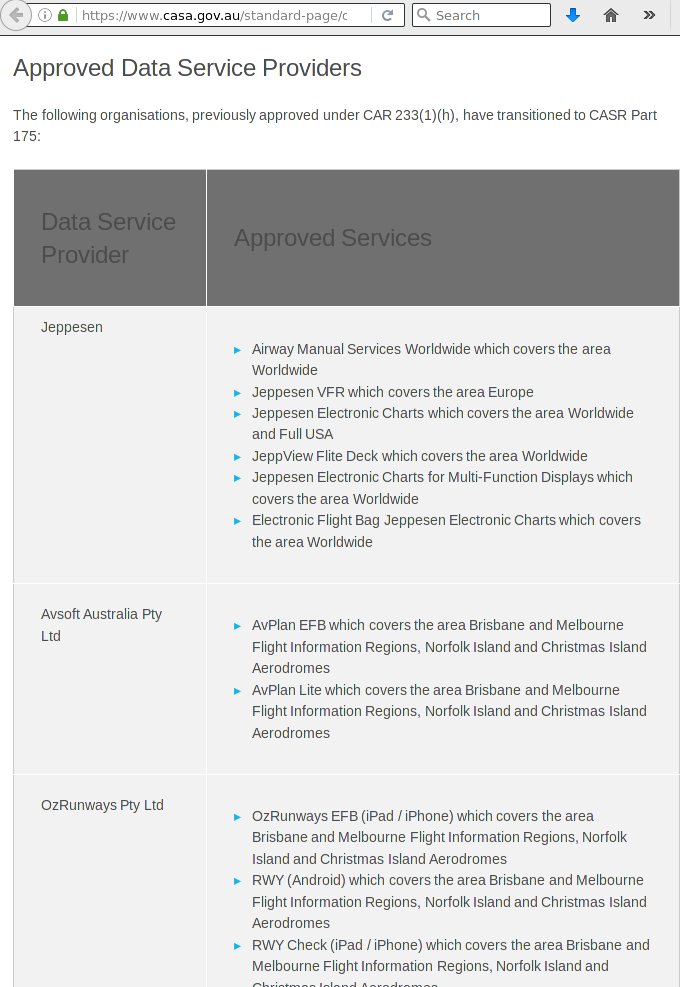
\includegraphics[height=0.8\textheight]{image/casa-approved-data-service-providers.png}
\end{center}
\end{frame}

\begin{frame}
\frametitle{CASR 175.145(1)}
\begin{block}{So then}
\begin{itemize}
\item<1-> I first came to terms with my deep resentment of legislated enforcement of proprietary hardware and software.
\item<2-> \ldots in safety-critical applications such as aviation.
\item<3-> I put aside my expectations of a complete failure.
\item<4-> I took a deep breath.
\end{itemize}
\end{block}
\end{frame}

\begin{frame}
\frametitle{CASR 175.145(1)}
\large
\begin{center}
and I installed ozrunways on a proprietary hardware device.
\end{center}
\end{frame}

\begin{frame}
\frametitle{CASR 175.145(1)}
\begin{center}
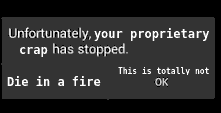
\includegraphics[height=0.2\textheight]{image/unfortunately-stopped.png}
\end{center}
\end{frame}

\begin{frame}
\frametitle{CASR 175.145(1)}
\begin{center}
\tiny{I am told that}
\par
\large
AvPlan fails at georectification.
\par
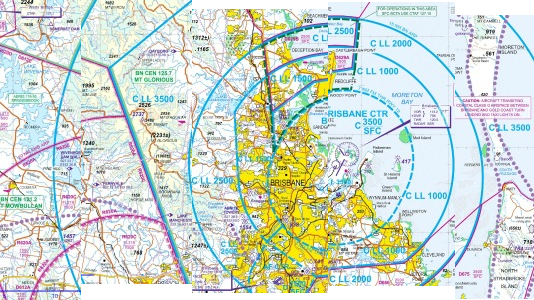
\includegraphics[height=0.5\textheight]{image/vtc-georectification.png}
\par
Knowingly and with no recourse to correct it.
\end{center}
\end{frame}

\begin{frame}
\frametitle{CASR 175.145(1)}
\begin{block}{Clearly then}
CASR 175.145(1) legislates forced use of unsafe, inferior aeronautical data.
\end{block}
\end{frame}

\begin{frame}
\frametitle{Civil Aviation Advisory Publication 233-1}
\begin{block}{CAAP 233-1 Electronic Flight Bags \emph{(excerpt)}}
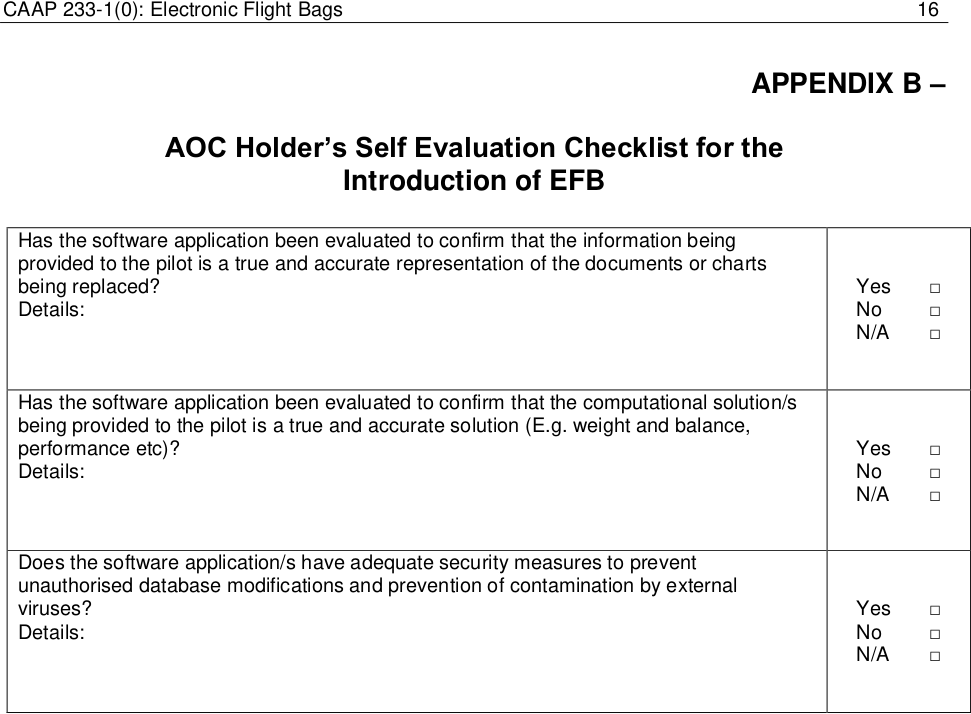
\includegraphics[height=0.6\textheight]{image/caap-233.png}
\end{block}
\end{frame}

\begin{frame}
\frametitle{CASR 175.145(1)}
\begin{center}

\includegraphics[height=0.5\textheight]{image/pls-halp.png}
\end{center}
\end{frame}
